\section{Part 3: Eye Movement Signal (EOG)}

\begin{taskbox}[Part 3: introduction in the lab manual]
A segment of EOG recorded from two channels (left eye and right eye) is provided in the file \texttt{sig\_EOG}.
\end{taskbox}

\subsection{Question 1: Displaying and Comparing the Two Channels and the Probable Recording Arrangement}
\begin{taskbox}
Plot the signals of the two channels versus time (seconds) and compare them with each other. Based on the signal shapes, sketch the approximate placement of the recording electrodes relative to the two eyes in a figure. What information can you obtain by visually inspecting the time-domain signal?
\end{taskbox}

The EOG data have two channels, left and right, with a sampling rate of 128~Hz and a duration of 60~s. Figure~\ref{fig:eog2ch} shows the complete recording and a zoomed common interval. Slow changes, relatively constant periods and fast transitions can be seen. In part of the recording the two channels have opposite trends, but the two versions are not completely inverted copies of each other; the raw correlation is about $-0.409$.

\begin{figure}[H]
\centering
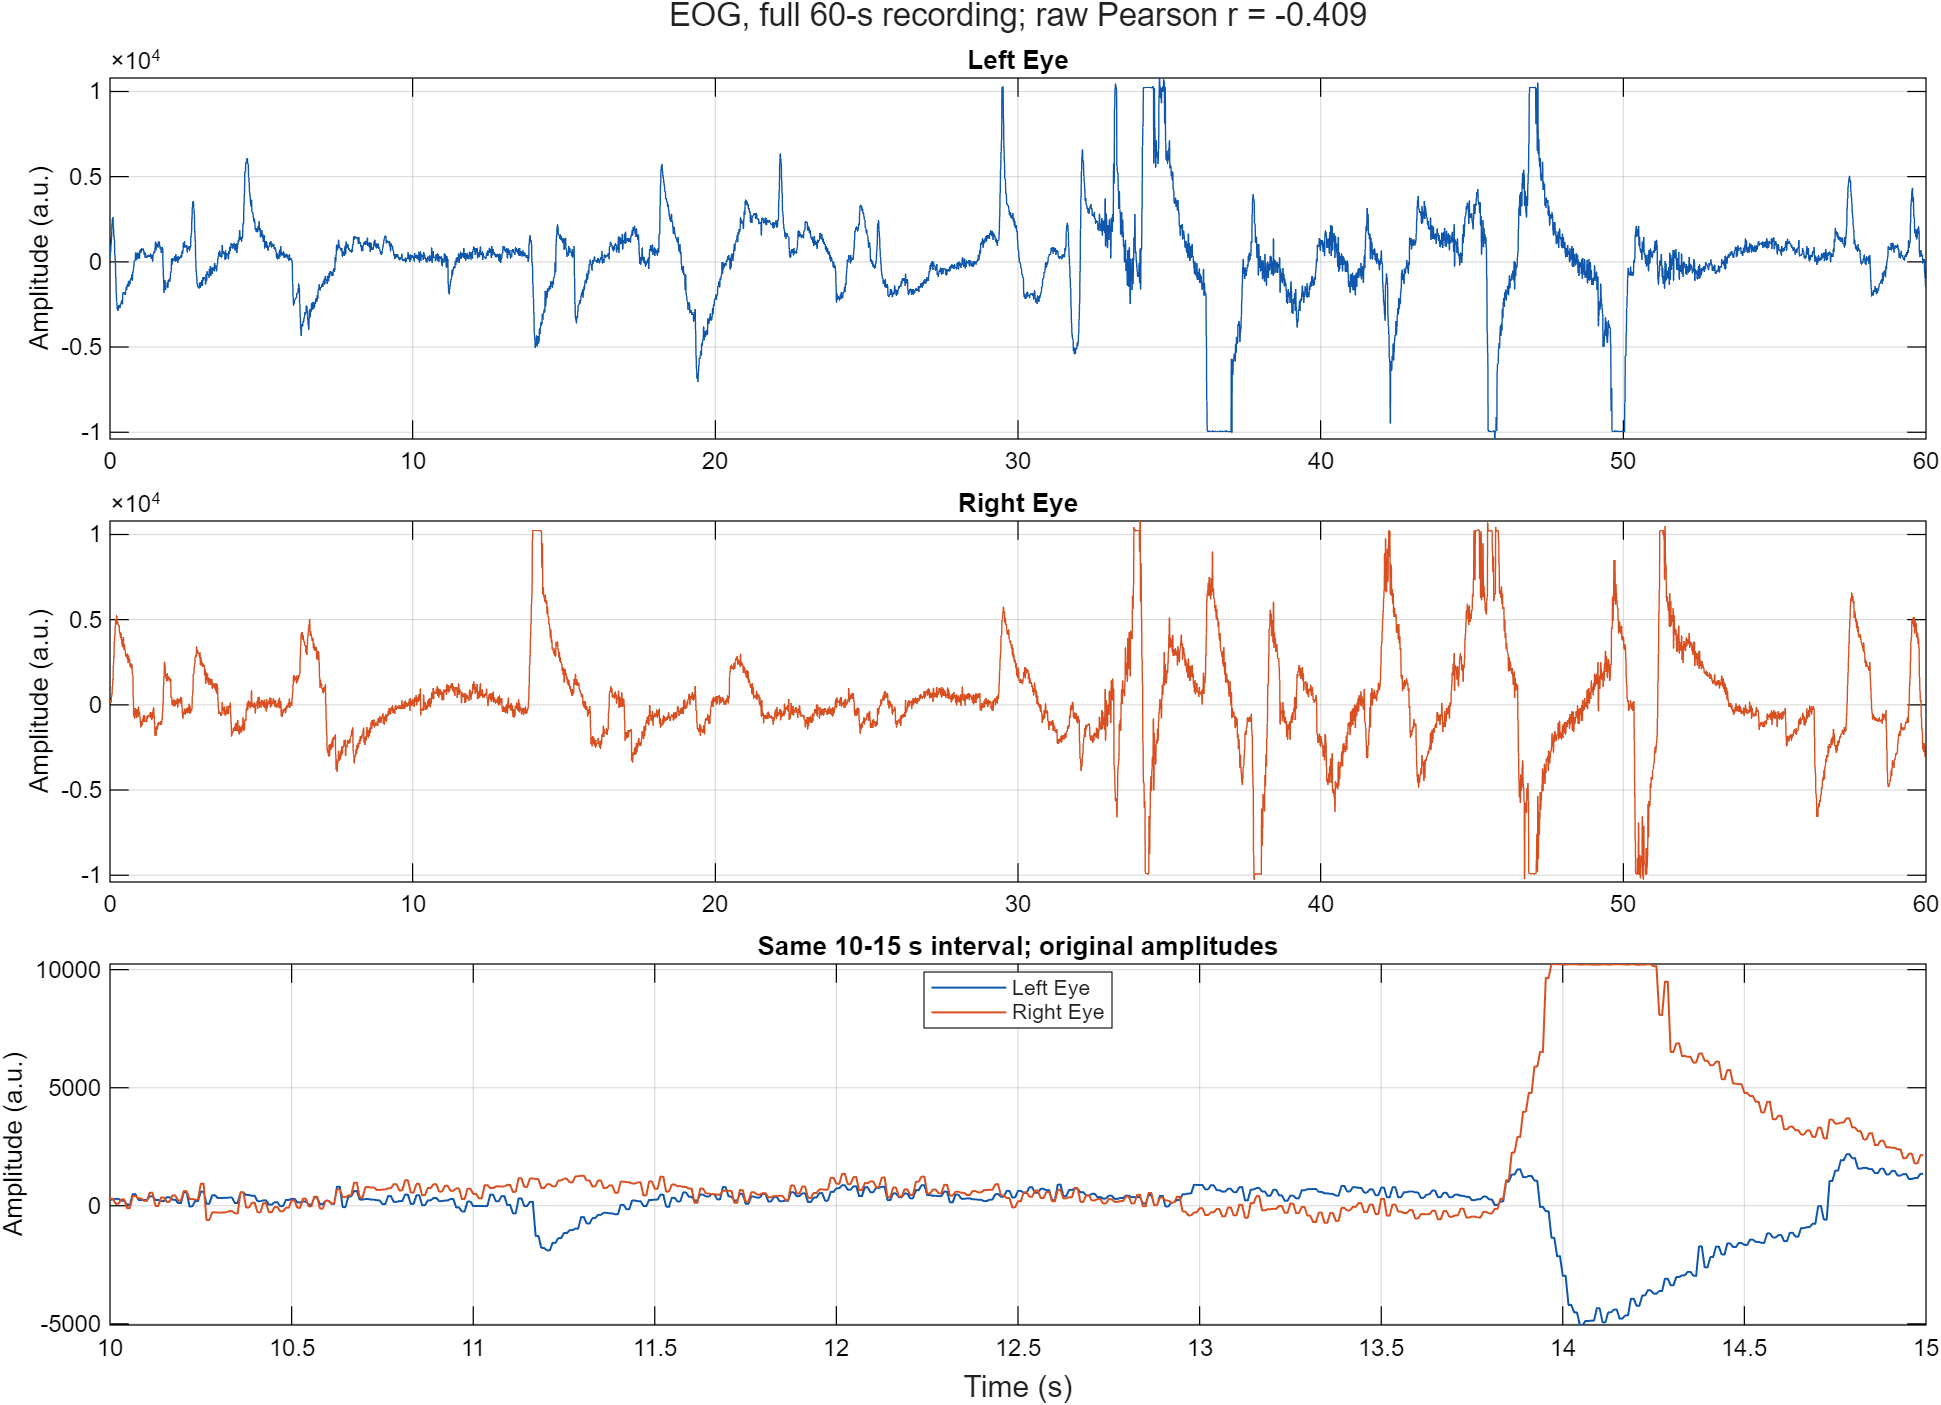
\includegraphics[width=0.95\textwidth]{fig20_eog_two_channels.png}
\caption{The two eye channels with common axes, and a zoom on the interval from ten to fifteen seconds.}
\label{fig:eog2ch}
\end{figure}

To describe the slow changes separately, a fourth-order Butterworth low-pass filter with a cutoff of 5~Hz, applied forward and backward, was used; this filter serves only for the comparison and does not replace the raw data. The correlation of the slow component is about $-0.424$, and the correlation of its derivative is about $-0.360$. Figure~\ref{fig:eogslow} emphasizes that both the trend and the timing of the transitions differ between the channels.

\begin{figure}[H]
\centering
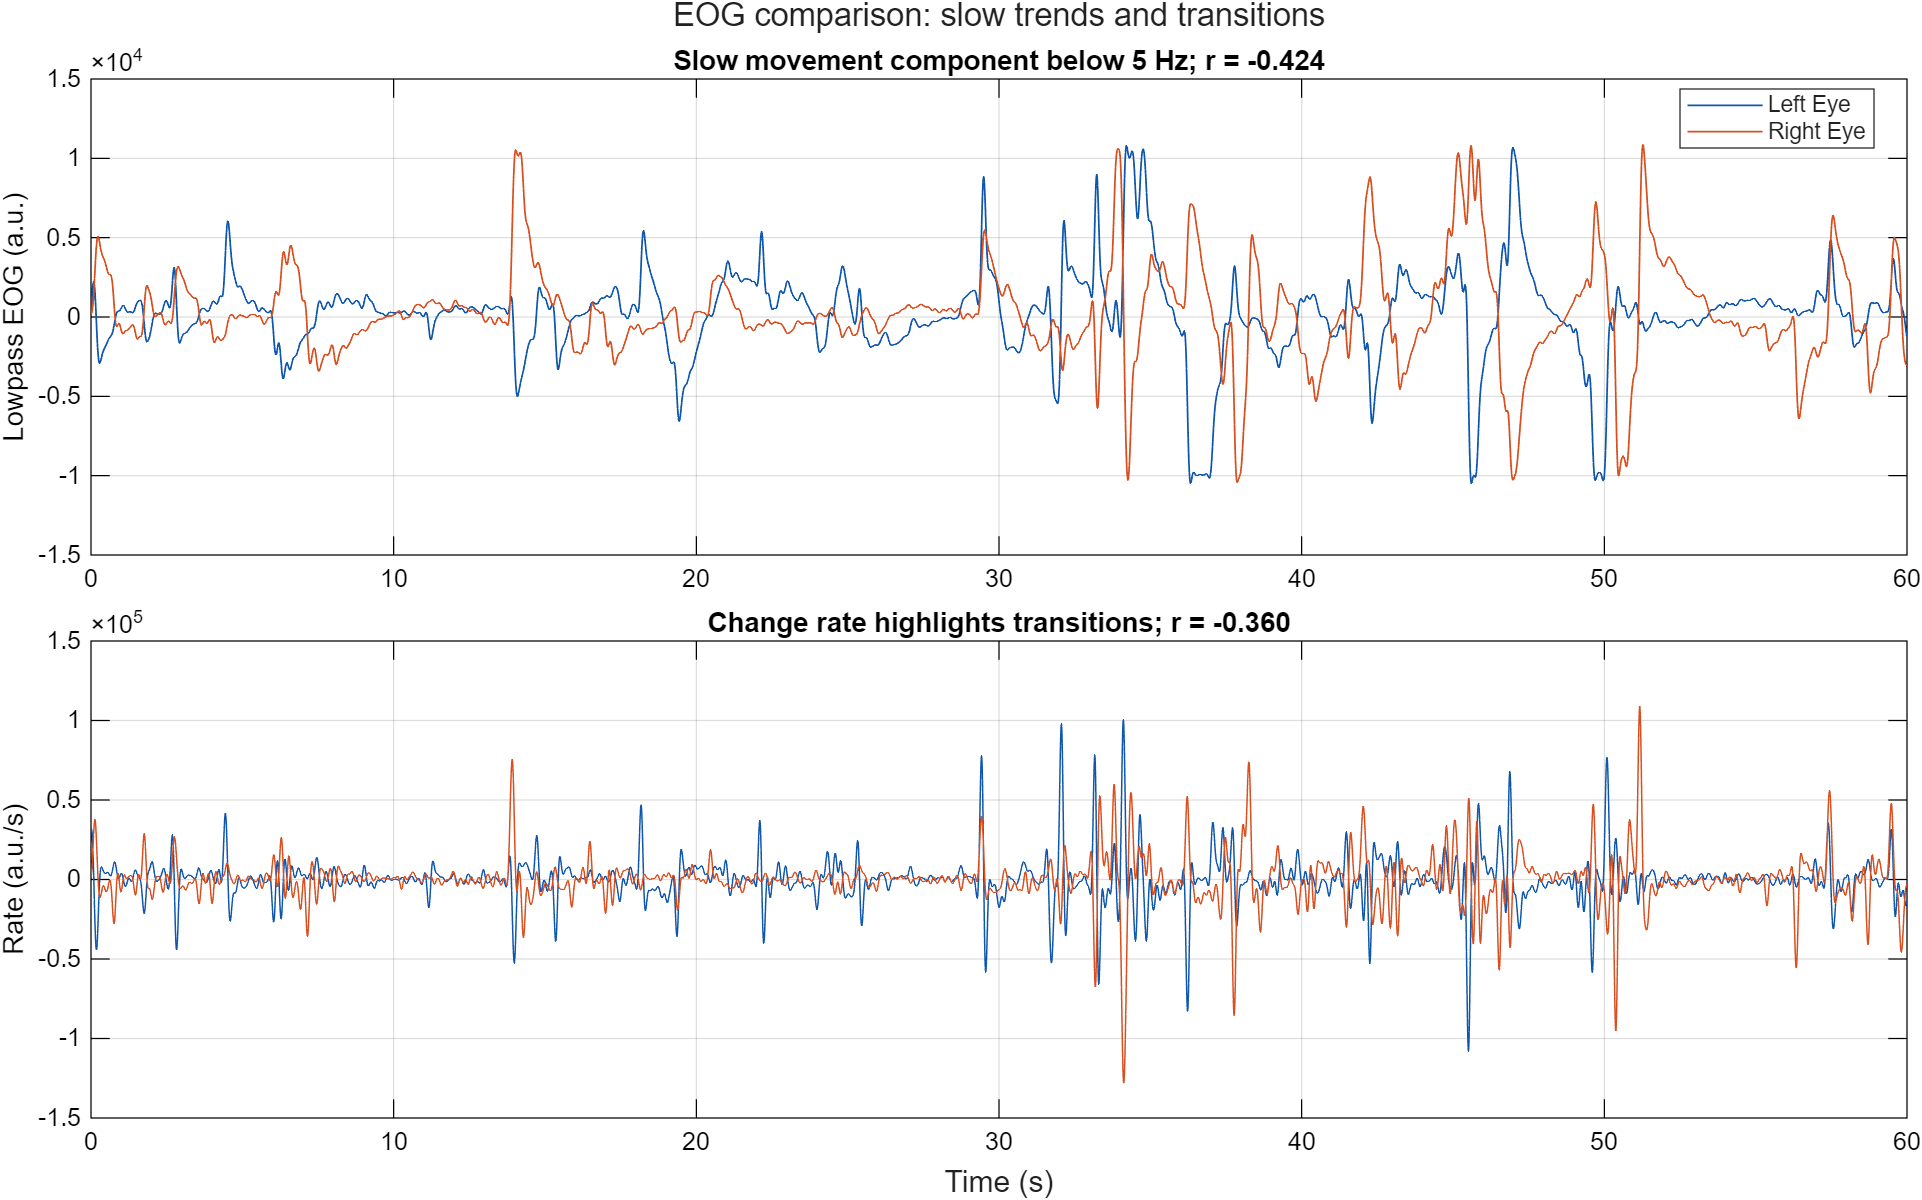
\includegraphics[width=0.95\textwidth]{fig21_eog_slow_trends_and_rate.png}
\caption{Comparison of the slow trends and their rates of change, for examining the timing of the eye transitions.}
\label{fig:eogslow}
\end{figure}

EOG recording relies on the potential difference between the cornea and the retina. An arrangement consistent with opposite changes in the two channels consists of lateral electrodes near the outer corners of the eyes and a common reference. Figure~\ref{fig:eogelec} shows this assumption from a frontal view; in this view, the left side of the person is on the right side of the image. From the two signals alone, the location of the reference, the exact locations of the electrodes or the polarity of the connection of the poles cannot be determined uniquely.

\begin{figure}[H]
\centering
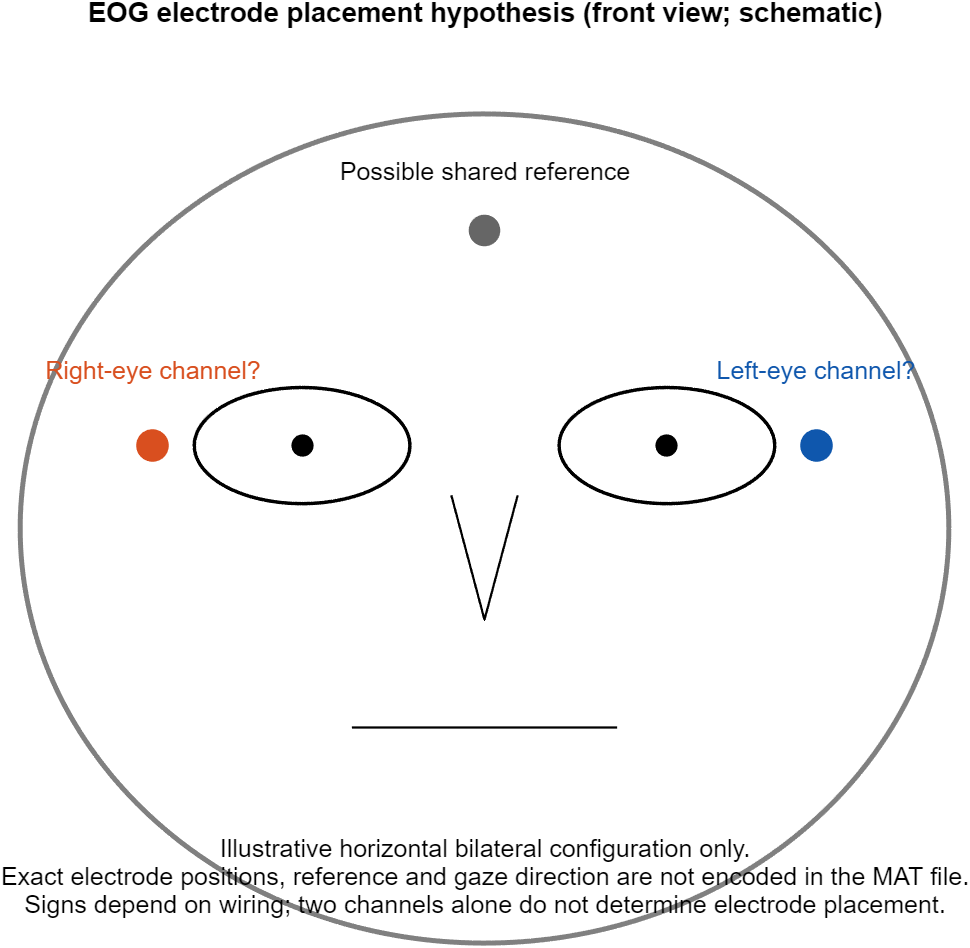
\includegraphics[width=0.6\textwidth]{fig22_eog_electrode_hypothesis.png}
\caption{A hypothetical lateral, horizontal arrangement of the electrodes for the eyes and the possible common reference.}
\label{fig:eogelec}
\end{figure}

From the time plot one can compare the timing and duration of the changes, the relative behavior of the two channels and the fast transitions. Determining the angle or the absolute direction of the gaze requires known calibration and polarity. Likewise, without a reference label, every fast transition cannot be called a blink or a saccade with certainty.

\subsection{Question 2: Frequency Spectrum and Spectrogram}
\begin{taskbox}
Plot the frequency spectrum and the time--frequency spectrum of the two channels and, based on them (and on the time-domain shape of the signals), explain the characteristics of the EOG signal.
\end{taskbox}

The one-sided Fourier transform was computed on the whole recording after removing the mean; the true spacing of its points is $1/60$~Hz. For Welch's method, a four-second Hann window, 75\% overlap and \texttt{nfft=2048} were used. According to Figure~\ref{fig:eogdft}, low-frequency components dominate. The integral of the power density below 5~Hz in both channels is about 98\% of the total Welch power.

\begin{center}
\begin{tabular}{@{}lccc@{}}
\toprule
\textbf{Channel} & \textbf{AC RMS} & \textbf{Power below 0.5~Hz (\%)} & \textbf{Power below 5~Hz (\%)}\\
\midrule
Left  & 2808.38 & 65.30 & 98.08\\
Right & 3058.52 & 58.01 & 98.00\\
\bottomrule
\end{tabular}
\end{center}

\begin{figure}[H]
\centering
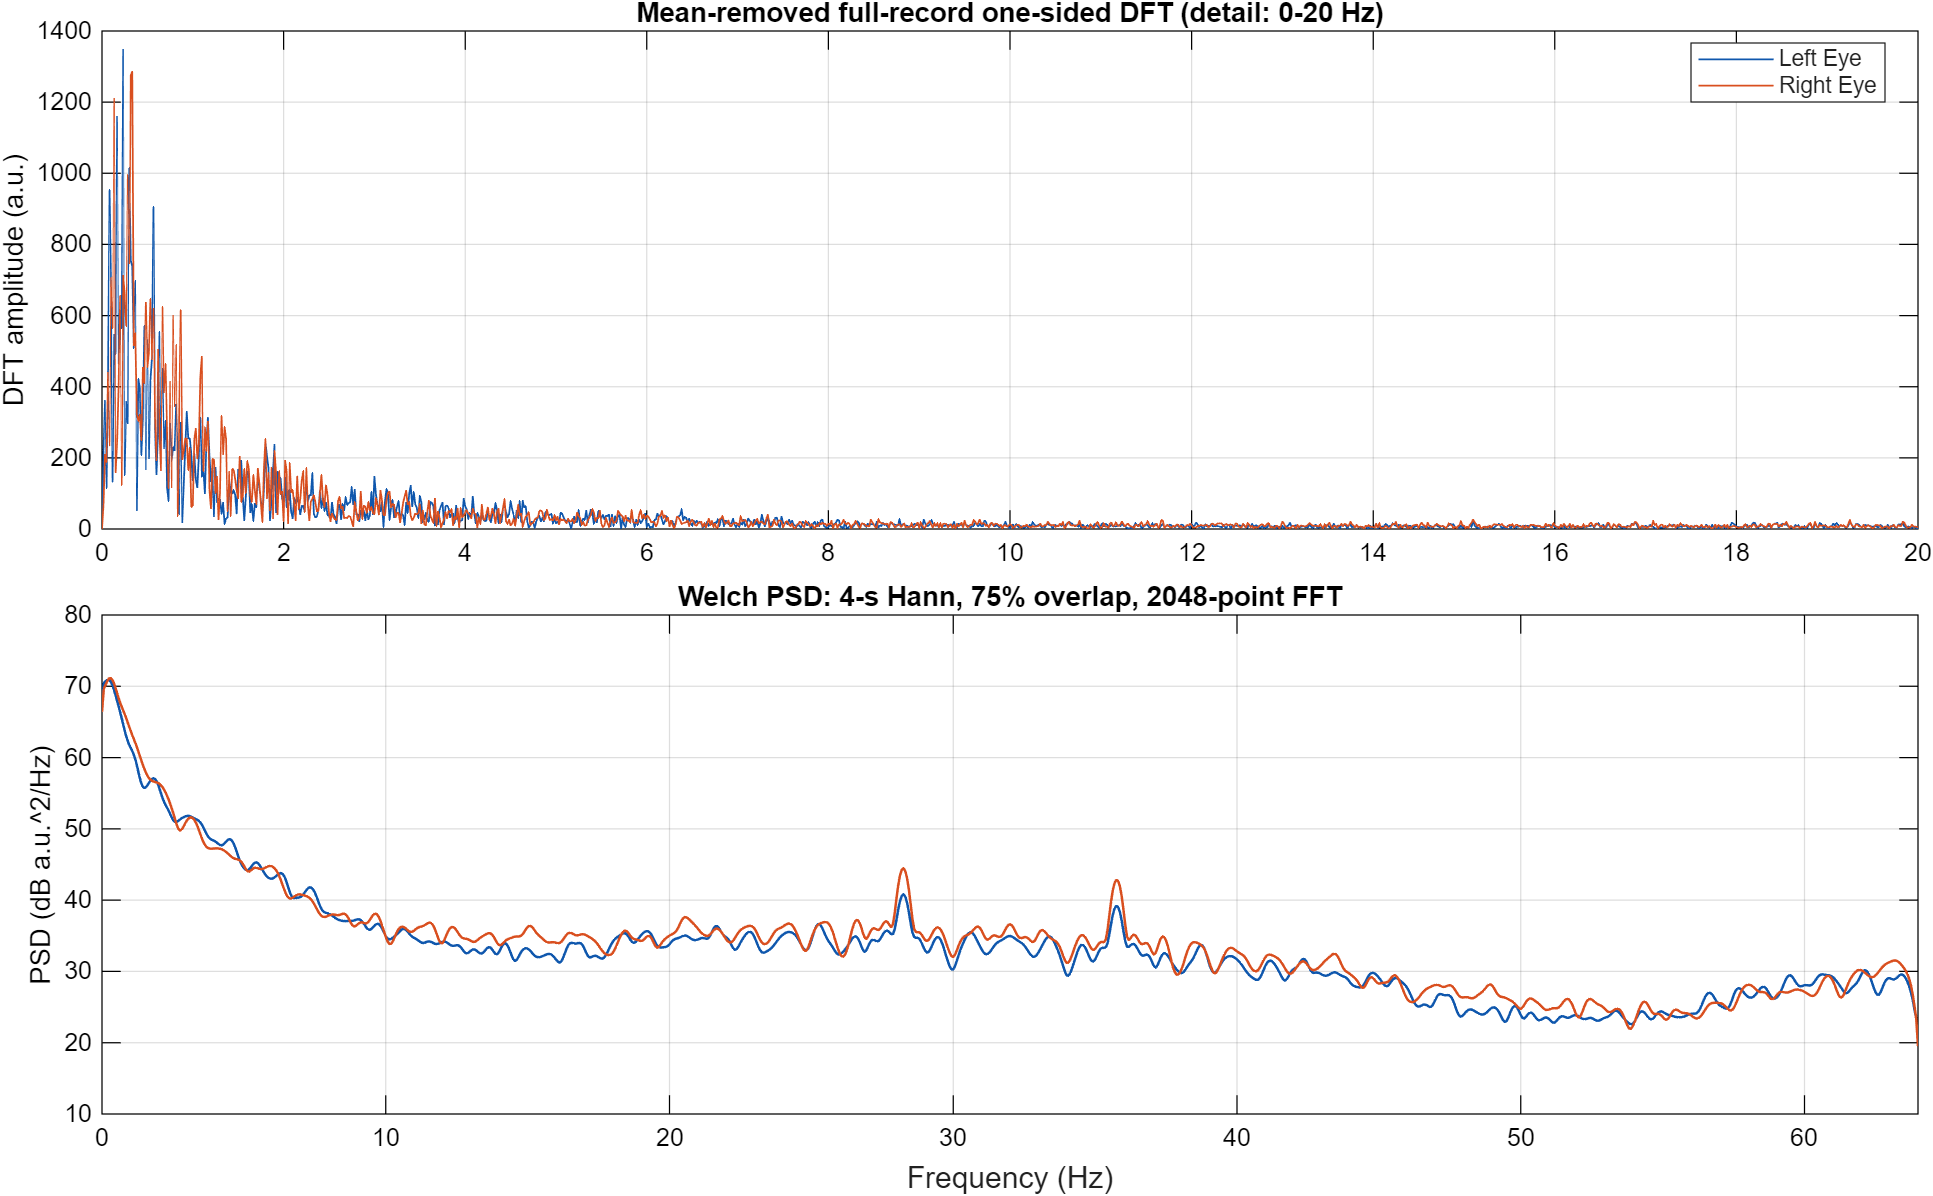
\includegraphics[width=0.95\textwidth]{fig23_eog_dft_and_psd.png}
\caption{Amplitude spectrum and power spectral density of the two eye channels, focusing on the low frequencies.}
\label{fig:eogdft}
\end{figure}

The dominance of low-frequency power is consistent with the slow changes of potential caused by eye displacement. Sharp transitions and noise can create broader energy. The RMS values of the left and right channels are close but not identical, and the peak-to-peak amplitudes of the two channels are 21168 and 21032~a.u., respectively.

For Figure~\ref{fig:eogstft}, a Hann window with a length of 256 samples, i.e.\ 2~s, an overlap of 224 samples and \texttt{nfft=1024} was used. The distribution of energy is not constant over time, and the transitions form regions of higher power at specific times. The overall spectrum shows the existence of low-frequency energy, but the spectrogram shows that this energy is not the same at all times. Faster components and noise are present alongside the dominant slow behavior.

\begin{figure}[H]
\centering
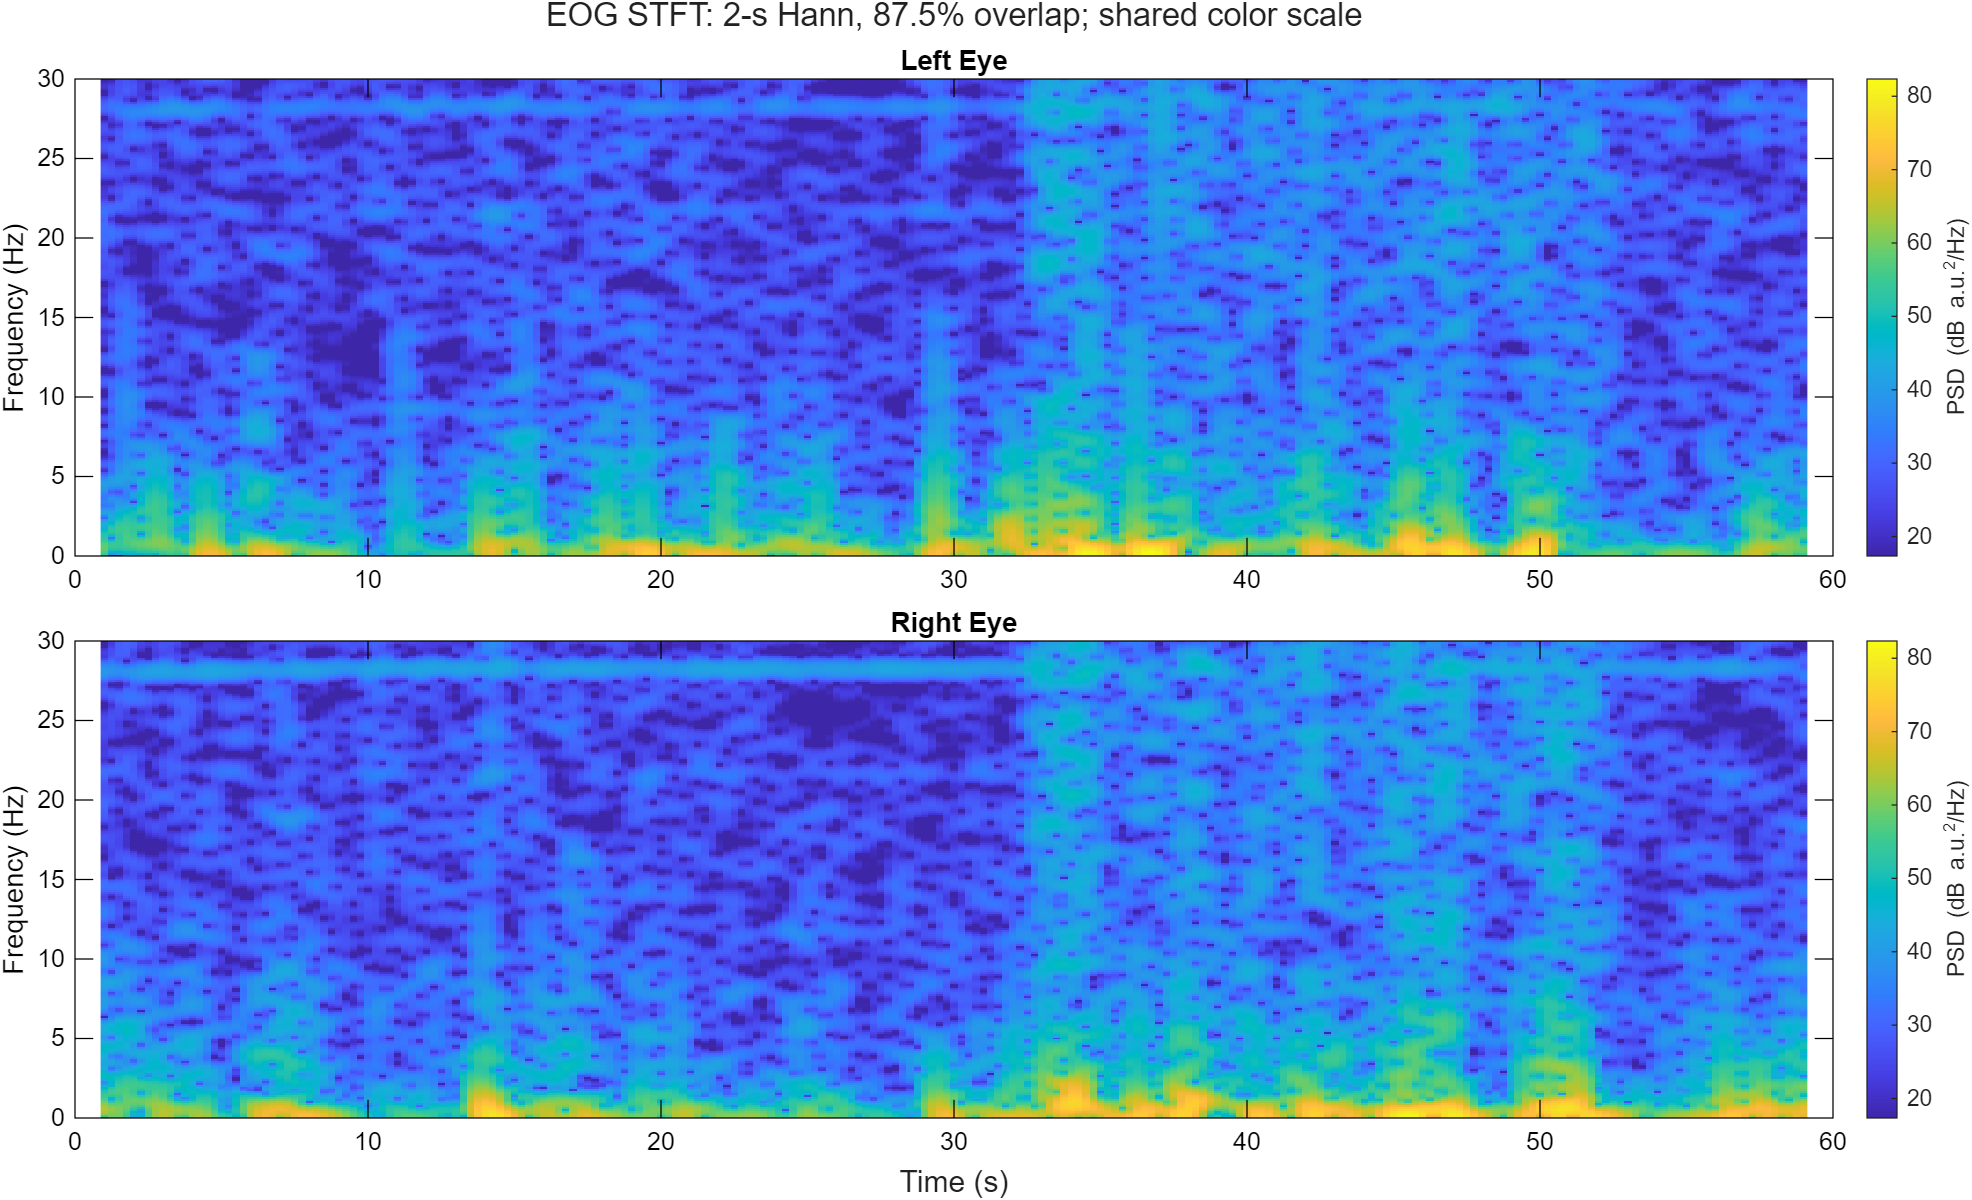
\includegraphics[width=0.95\textwidth]{fig24_eog_stft.png}
\caption{Spectrogram of the two eye channels with a common color scale, showing the temporal variations of the energy.}
\label{fig:eogstft}
\end{figure}

\subsection{Core Implementation (EOG)}

\begin{lstlisting}[language=Matlab]
t = (0:size(Sig,2)-1)/fs;
X = Sig-mean(Sig,2);
[P,f] = pwelch(X(1,:),hann(512,'periodic'),384,2048,fs);
[S,F,T,Ptf] = spectrogram(X(1,:),hann(256,'periodic'),224,1024,fs);
\end{lstlisting}

In this file the channels are rows; paying attention to this orientation prevents building an incorrect time axis or taking the Fourier transform along the channel axis. The complete implementation, together with the figure of the electrode arrangement, is in \texttt{code/lab1\_eog\_emg.m}.
